\documentclass[tikz,border=5pt]{standalone}
\usepackage{pgfplots}
\pgfplotsset{compat=1.18}

\begin{document}

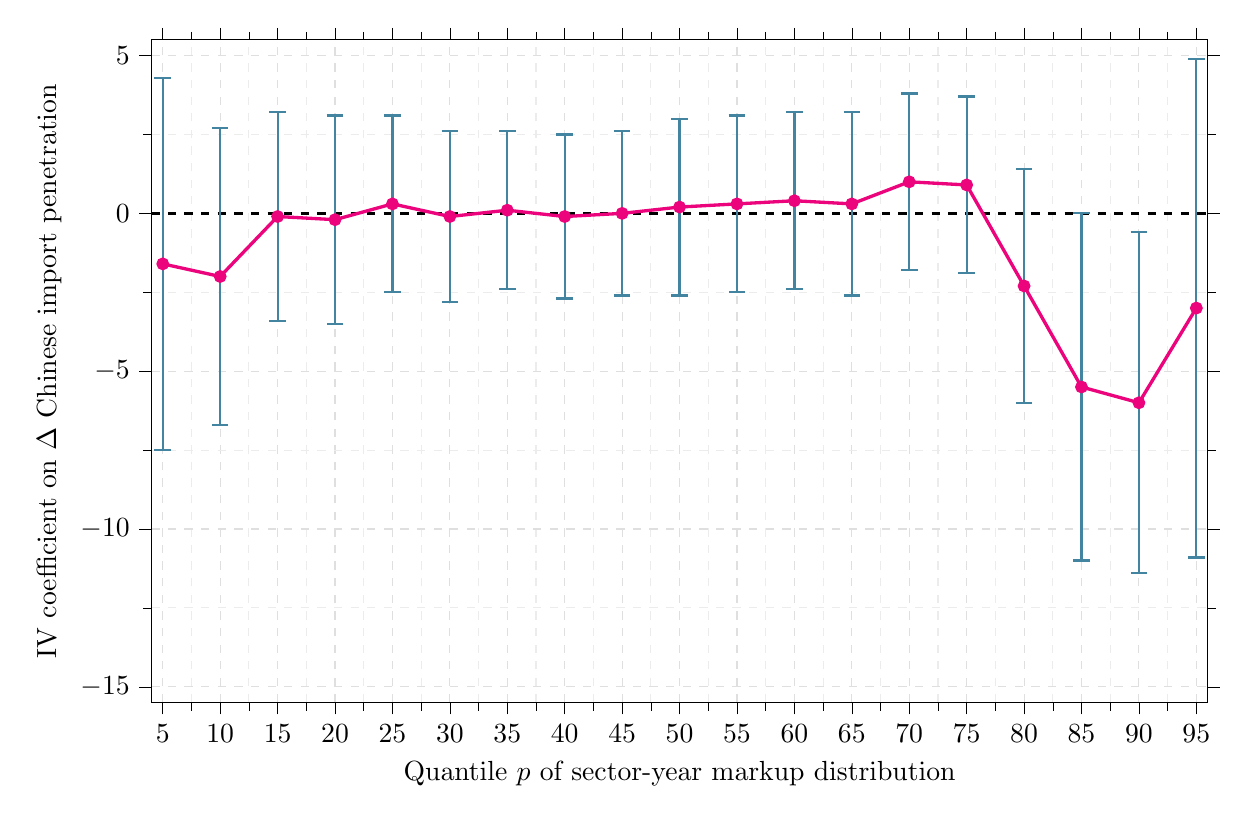
\begin{tikzpicture}
\begin{axis}[
    width=15cm,
    height=10cm,
    xmin=4, xmax=96,
    ymin=-15.5, ymax=5.5,
    xtick={5,10,15,20,25,30,35,40,45,50,55,60,65,70,75,80,85,90,95},
    ytick={-15,-10,-5,0,5},
    xlabel={Quantile $p$ of sector-year markup distribution},
    ylabel={IV coefficient on $\Delta$ Chinese import penetration},
    axis line style={black},
    tick style={black},
    tick align=outside,
    grid=both,
    major grid style={dashed,draw=gray!25},
    minor grid style={dashed,draw=gray!15},
    minor x tick num=1,
    minor y tick num=1,
    enlargelimits=false,
    clip=false
]

% horizontal dashed zero line
\addplot[
    black,
    dashed,
    line width=0.9pt
] coordinates {(4,0) (96,0)};

% error bars + points
\addplot[
    only marks,
    mark=*,
    mark size=1.5pt,
    color=cyan!60!black,
    error bars/.cd,
    y dir=both,
    y explicit,
    error bar style={line width=0.8pt, color=cyan!60!black},
    error mark options={rotate=90, mark size=3pt, line width=0.8pt, color=cyan!60!black}
] coordinates {
    (5,  -1.6) +- (0, 5.9)
    (10, -2.0) +- (0, 4.7)
    (15, -0.1) +- (0, 3.3)
    (20, -0.2) +- (0, 3.3)
    (25,  0.3) +- (0, 2.8)
    (30, -0.1) +- (0, 2.7)
    (35,  0.1) +- (0, 2.5)
    (40, -0.1) +- (0, 2.6)
    (45,  0.0) +- (0, 2.6)
    (50,  0.2) +- (0, 2.8)
    (55,  0.3) +- (0, 2.8)
    (60,  0.4) +- (0, 2.8)
    (65,  0.3) +- (0, 2.9)
    (70,  1.0) +- (0, 2.8)
    (75,  0.9) +- (0, 2.8)
    (80, -2.3) +- (0, 3.7)
    (85, -5.5) +- (0, 5.5)
    (90, -6.0) +- (0, 5.4)
    (95, -3.0) +- (0, 7.9)
};

% magenta line with points
\addplot[
    color=magenta!85!red,
    line width=1.2pt,
    mark=*,
    mark size=1.7pt,
    mark options={fill=magenta!85!red, draw=magenta!85!red}
] coordinates {
    (5,  -1.6)
    (10, -2.0)
    (15, -0.1)
    (20, -0.2)
    (25,  0.3)
    (30, -0.1)
    (35,  0.1)
    (40, -0.1)
    (45,  0.0)
    (50,  0.2)
    (55,  0.3)
    (60,  0.4)
    (65,  0.3)
    (70,  1.0)
    (75,  0.9)
    (80, -2.3)
    (85, -5.5)
    (90, -6.0)
    (95, -3.0)
};

\end{axis}
\end{tikzpicture}

\end{document}



\end{document}